\begin{frame}{Computations on Honeycomb FBI}
\vskip-1.5cm
\begin{columns}[T]
    \begin{column}[T]{.5\textwidth}
 	    \only<1>{
 	    \begin{figure}
			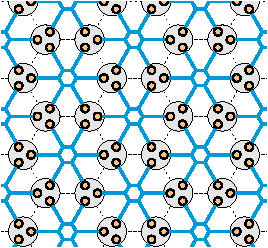
\includegraphics[width=\textwidth]{diagrams/FI_PEPS.pdf}
			\end{figure}
			$$
			\ket{\psi} = \prod\limits_{\varhexagon} \left(\sum\limits_{i \in \varhexagon} b^{\dagger}_i \right) \ket{\mathbf{0}}
			$$ 
		}
		\only<2->{
			\begin{figure}
				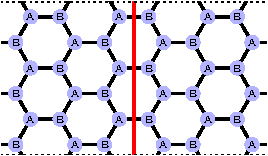
\includegraphics[width=\textwidth]{diagrams/Hex_PEPS.pdf}
				\caption{Form of a honeycomb lattice PEPS on zig-zag cylinder with width L=3}
			\end{figure}
		}
		\only<3->{
			\begin{figure}
				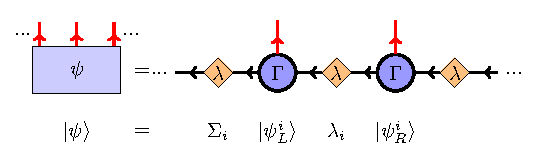
\includegraphics[width=\textwidth]{diagrams/mps_canonical.pdf}
				\caption{Matrix Product state canonical form}
			\end{figure}
		}
    \end{column}
    \begin{column}[T]{.5\textwidth}
		\bi
		\item<1->[] Simple tensor network representation
		\item<2->[] Cylinder slice treated as single site of an effective 1D system.
		\item<3->[] Schmidt decomposition computed as in 1D matrix product states.
		\ei	
    \end{column}
\end{columns}
\end{frame}